\begin{figure*}[t]
\centering
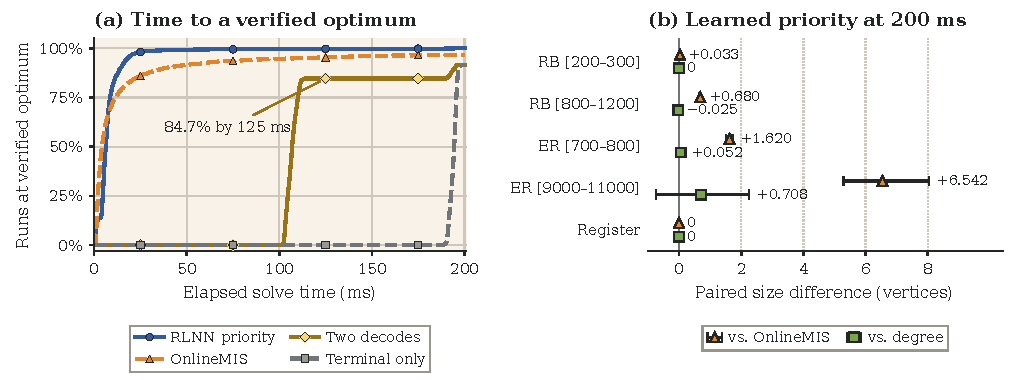
\includegraphics[width=1.0\textwidth]{figures/intro_evidence.pdf}
\caption{\textbf{Delivery timing and the effect of learning.}
(a) Curves show the share of 3,000 small RB graph--seed pairs with an offline-verified optimum already on the host. The particle clock starts at per-graph buffer loading and the resident clock at the host edge list. By 125~ms, two decodes deliver 2,540 optima and terminal-only decoding delivers none. Both reach 2,750 by 200~ms.
(b) Points show learned priority minus each comparator in mean delivered size at 200~ms. Whiskers give pointwise 95\% graph-bootstrap intervals. Small ER uses the single-core interleaved repeat. All three methods tie on every seed of the 14 register graphs. Legend labels: ``RLNN priority'' is the learned ranking of SPRINT-C.}
\label{fig:intro-evidence}
\end{figure*}
